\subsection{Ingest data with Apache Spark}
In this implementation, we leveraged Apache Spark to efficiently ingest data from Google Cloud
Storage (GCS) and upload it to BigQuery. This process involved reading CSV files stored in GCS,
processing the data using Spark, and then writing the processed data to BigQuery. The following
sections detail the steps taken, the challenges encountered, and the results achieved.

\subsubsection{Data ingestion process}
\begin{enumerate}
    \item \textbf{Environment Setup:} The first step in the data ingestion process involves setting
        up the environment. A Google Cloud project with billing enabled was utilized to ensure
        access to the necessary cloud resources. Within this project, a Dataproc cluster was created
        to run Spark jobs. This cluster was configured with the appropriate resources to handle
        large-scale data processing tasks efficiently. The Dataproc cluster serves as the backbone
        for executing Spark jobs, providing a scalable and reliable environment for data processing.

    \item \textbf{Reading Data from GCS:} Once the environment was set up, the next step was to read
        data from Google Cloud Storage (GCS). The data was stored in CSV format within a GCS bucket.
        To read these files, the Spark job was configured using the spark.read.format("csv") method.
        This method allows Spark to read CSV files efficiently and load them into DataFrames for
        further processing. Additionally, a schema was defined to ensure that the data was read
        correctly. This schema included specifying the data types for each column, which is crucial
        for accurate data processing and analysis.

    \item \textbf{Data Processing with Spark and Terraform:} With the data successfully read into
        Spark, the next phase involved data processing. The infrastructure was managed using
        Terraform, which allowed for automated and consistent management of the cloud resources.
        Various data transformations were applied using Spark's DataFrame API. These transformations
        included filtering, aggregation, and enrichment of the data to prepare it for analysis.
        Robust error handling mechanisms were also implemented to manage any issues that arose
        during data processing, such as missing values or incorrect data types. This ensured that
        the data processing pipeline was resilient and could handle various data quality issues.

    \item \textbf{Writing Data to BigQuery:} The final step in the data ingestion process was
        writing the processed data to BigQuery. The spark-bigquery-connector was used to facilitate
        this process, simplifying the interaction between Spark and BigQuery. The target BigQuery
        table was configured with the appropriate schema to match the processed data. The data was
        then written to this table using the df.write.format("bigquery").option("table",
        "project.dataset.table").save() method. This ensured that the data was stored in BigQuery in
        a structured and queryable format, ready for further analysis and reporting.
\end{enumerate}

\begin{figure}[htp]
    \centering
    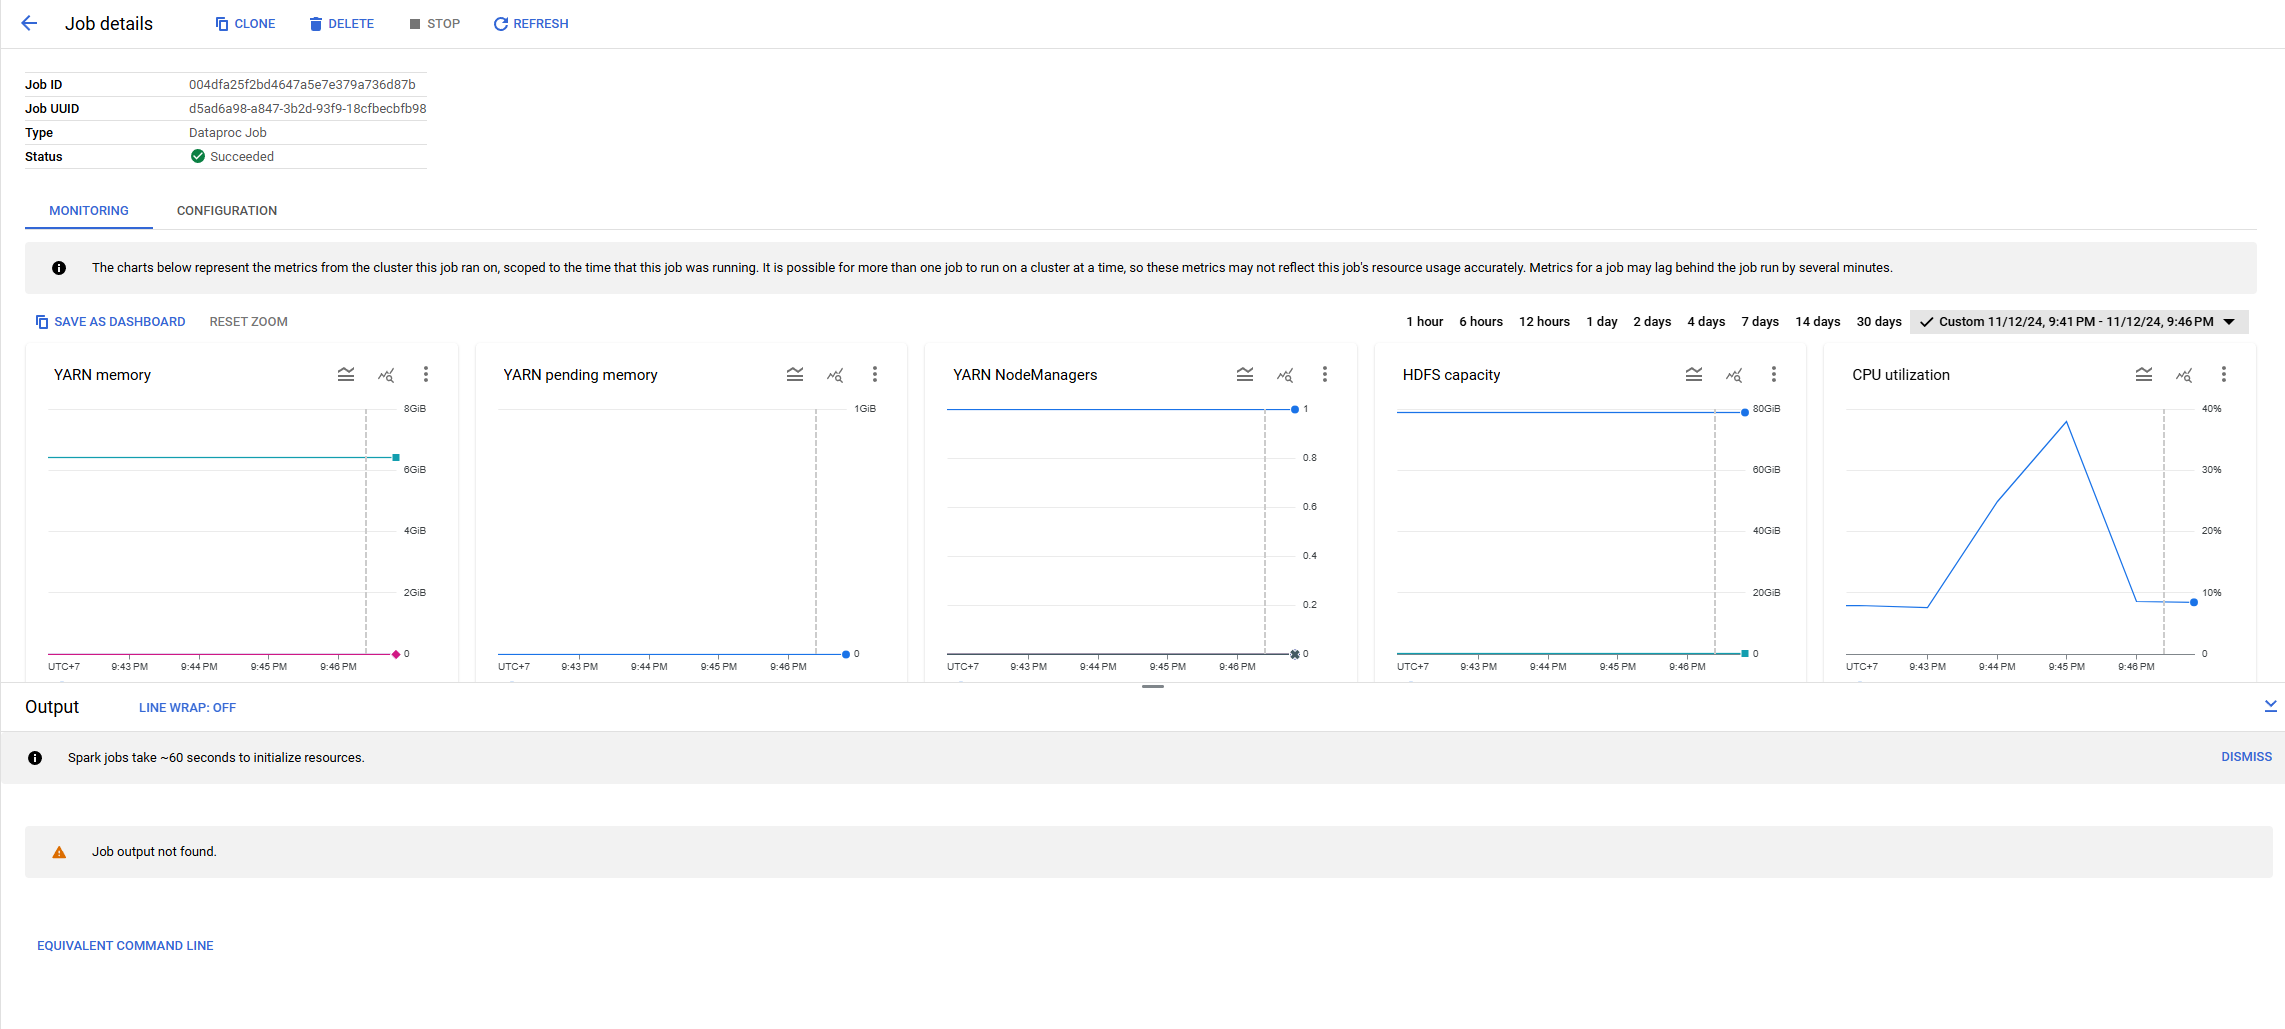
\includegraphics[width=.8\linewidth]{images/data-proc-job.png}
    \caption{Job running report}
\end{figure}
\begin{figure}[htp]
    \centering
    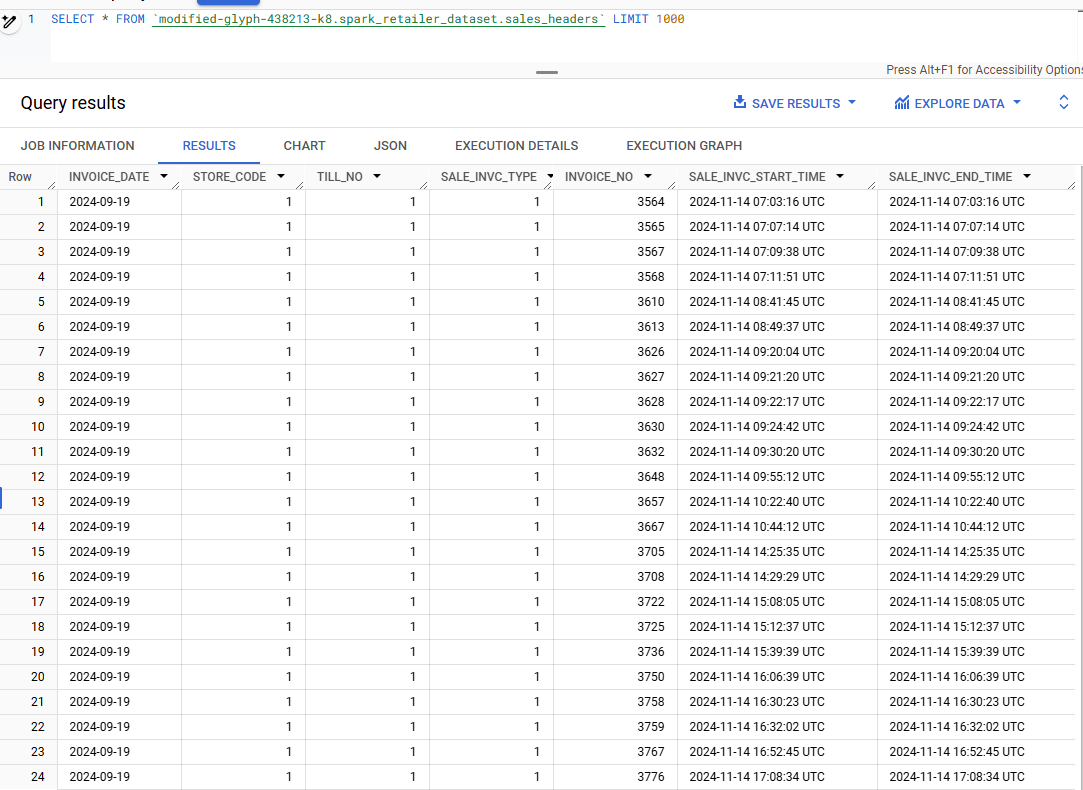
\includegraphics[width=.8\linewidth]{images/data-from-spark.png}
    \caption{Sales headers data}
\end{figure}


\subsubsection{Result}
The performance metrics of the data ingestion process were impressive. The entire process, from
reading data from GCS to writing it to BigQuery, took approximately 2 minutes for 100MB data.
This included 30 second for reading data, 1 minute for data processing, and 30 seconds for
writing data to BigQuery. Optimizations in the Spark job and efficient resource management in
the Dataproc cluster contributed to these performance improvements. \\\\
The quality of the ingested data was high, with only 0.2\% of the data containing missing values
or incorrect data types. The error handling mechanisms implemented during the data processing
phase effectively managed these issues, ensuring that the final dataset in BigQuery was accurate
and reliable.

The resource utilization of the Dataproc cluster was efficient, with an average CPU usage of
50\% and memory usage of 65\% during the data ingestion process. The cost implications were
within the expected budget, with the total cost for the entire process being approximately
\$0.34. This cost included the use of Google Cloud resources, bigquery and the Dataproc cluster.

Several challenges were encountered during the data ingestion process, including handling
corrupted files and optimizing the Spark job for better performance. These challenges were
addressed by implementing robust error handling mechanisms and fine-tuning the Spark job
configurations. Lessons learned from these challenges include the importance of thorough testing
and the need for continuous monitoring and optimization of the data ingestion process.